\section{Realizzazione}
Ogni pagina ha un suo scheletro in un file HTML, il quale viene aperto dal file \textit{nome\textunderscore pagina.php} tramite la funzione \textit{file\textunderscore get\textunderscore contents()}, successivamente la pagina viene popolata dalla classe PHP \textbf{htmlMaker} da noi sviluppata e solo a questo punto viene mostrata all'utente.\\
Così facendo riusciamo a tenere totalmente separato il comportamento dalla struttura, riusciamo a gestire le sessioni e non abbiamo bisogno di fare chiamate AJAX dalle pagine.
\subsection{HTML}
Abbiamo cominciato scrivendo un header e un footer che fossero unici per tutte le pagine, questi due file HTML vengono letti dalla classe \textit{htmlMaker} e inseriti in tutte le pagine presenti nel sito. Successivamente abbiamo iniziato a scrivere il codice HTML di ogni altra pagina, a partire dalla home, prodotti e contatti. Man mano che le pagine prendevano forma andavamo a spostare il codice HTML scritto, nella classe PHP responsabile della generazione del contenuto delle varie pagine.
\subsection{CSS}
Riguardo allo stile CSS, abbiamo lavorato parallelamente allo sviluppo delle pagine, a partire dallo stile principale condiviso per poi procedere anche con lo stile per dispositivi mobile, la quale presentazione è gestita da un apposito foglio di stile che ottimizza la visualizzazione e dispone barra di navigazione e pulsanti di ricerca e account nel menu ad hamburger nella parte destra dell'header.


\begin{figure}[H]
	\centering
	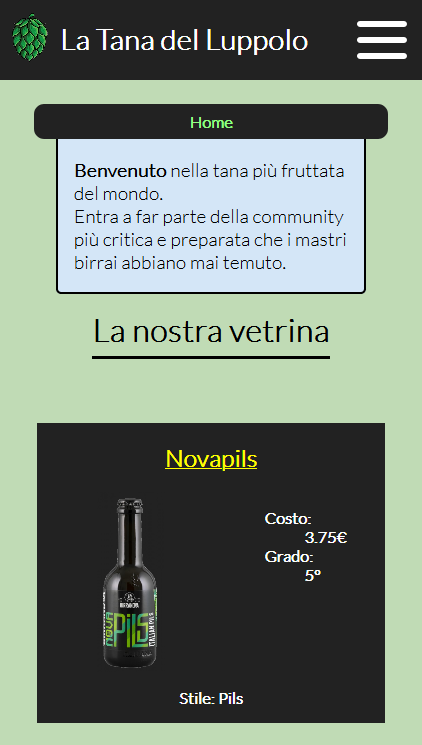
\includegraphics[width=6cm]{utility/home_mobile.png}
	\caption{Il layout mobile della homepage}
\end{figure}

\pagebreak

Infine è stato predisposto un foglio di stile per la stampa dalla quale sono stati nascosti alcuni elementi giudicati superflui (ad esempio la barra di navigazione o i pulsanti back-to-top-button, ricerca e account) o modificati per migliorarne la presentazione (come la breadcrumb, le recensioni o la grandezza delle immagini principali).

\begin{figure}[H]
	\centering
	\caption{Il layout di stampa della pagina Prodotti}
	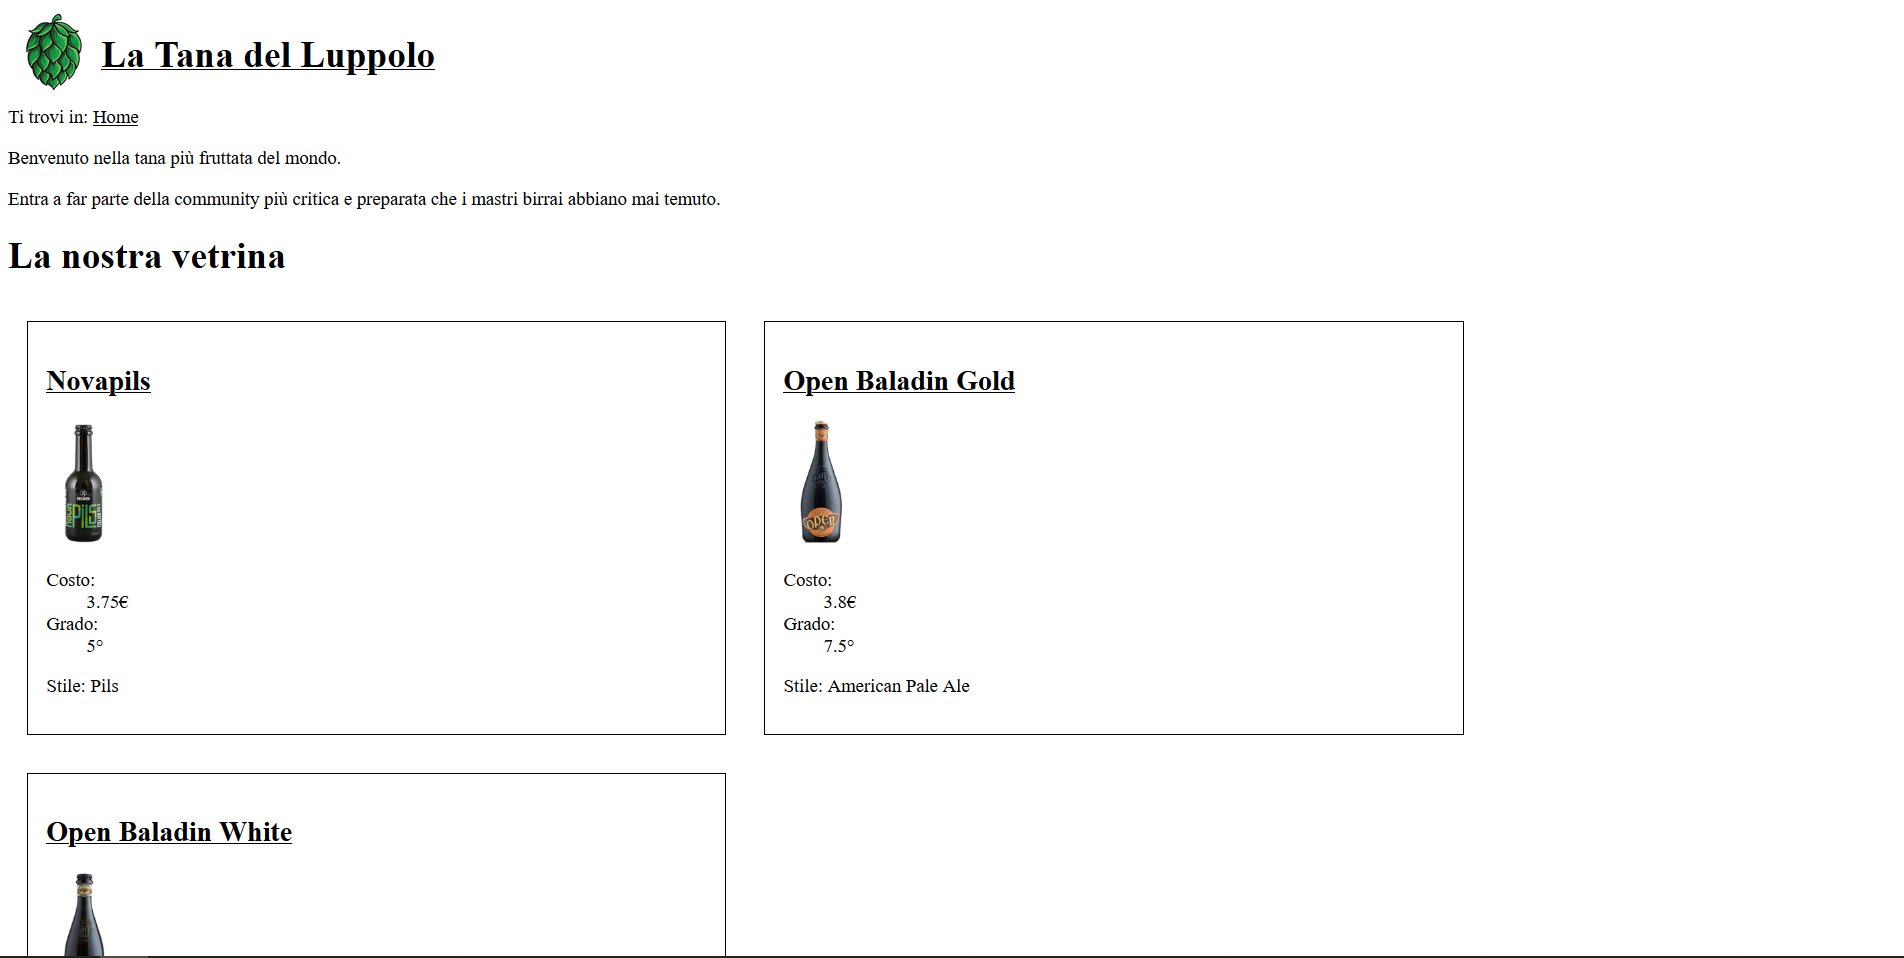
\includegraphics[width=16cm]{utility/prodotti_printcss.png}
\end{figure}

I colori dominanti del sito sono il grigio scuro e un verde pistacchio per header, sfondi ed altri elementi di presentazione mentre vengono utilizzati il nero, il verde ed il giallo per testi e link.\\

% palette colori
Sfondi ed elementi
\definecolor{hdgray}{RGB}{34, 34, 34}
\definecolor{pistacho}{RGB}{192, 219, 181}
\definecolor{puffo}{RGB}{212, 230, 247}
\crule[hdgray]{1cm}{1cm} \crule[pistacho]{1cm}{1cm} \crule[puffo]{1cm}{1cm} 


Testi e link
\definecolor{bcgreen}{RGB}{167, 255, 131}
\definecolor{hdgreen}{RGB}{216, 251, 216}
\crule{1cm}{1cm} \crule[yellow]{1cm}{1cm} \crule[bcgreen]{1cm}{1cm} \crule[hdgreen]{1cm}{1cm}
\\

La palette è stata scelta in modo da garantire una corretta visualizzazione anche da persone affette da diversi tipi di cecità o sensibilità del contrasto ed il contenuto del sito rimane correttamente visualizzabile anche senza il caricamento dello stile CSS.

\begin{figure}[H]
	\centering
	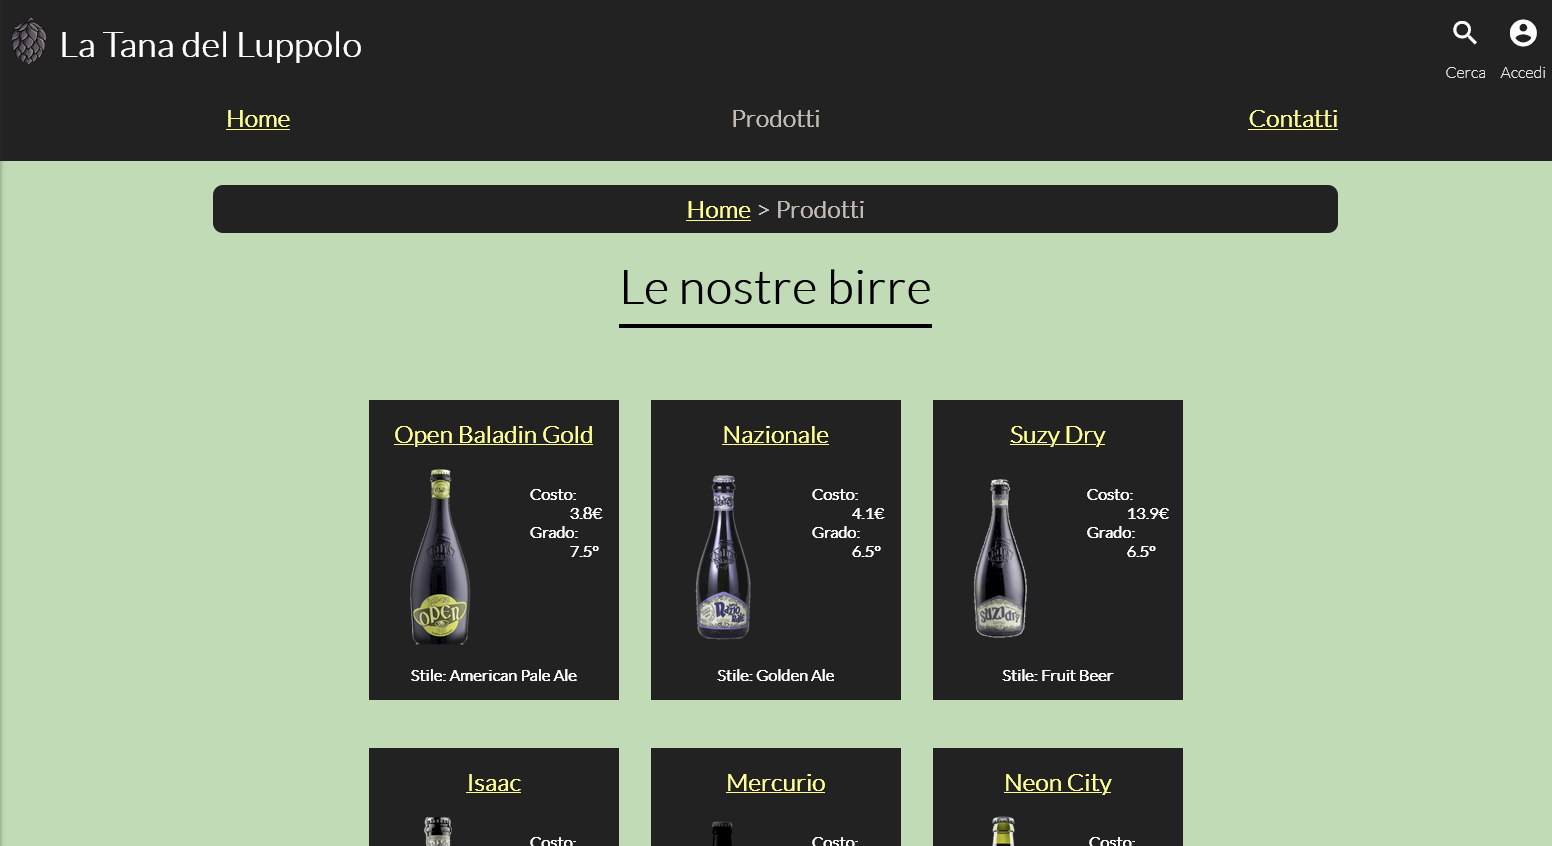
\includegraphics[width=16cm]{utility/prodotti_deuteranopia.png}
	\caption{Vista della pagina Prodotti da persone affette da deuteranopia (cecità al verde)}
\end{figure}


\subsection{Javascript}
\subsection{PHP}
Nel nostro sito, ogni pagina é generata da un file PHP.
Abbiamo creato due classi con metodi statici,una per la costruzione dell'html e una per la connessione al database, abbiamo deciso di utilizzare solo metodi statici in mod da non dover istanziare oggetti per richiamarne le funzioni:
\begin{itemize}
\item \textbf{htmlMaker.php:} si occupa della costruzione di codice html, ed é composta dai seguenti metodi:
	\begin{itemize}
		\item \textit{makeHead}: metodo utilizzato da tutte le pagine del sito, costruisce l'head html.
		\item \textit{makeHeader}: metodo utilizzato da tutte le pagine del sito, costruisce l'intestazione html.
		\item \textit{makeHeading}: metodo utilizzato da tutte le pagine del sito, costruisce il titolo principale.
		\item \textit{makeBreadCrumbs}: metodo utilizzato da tutte le pagine del sito, costruisce la breadcrumb.
		\item \textit{makeTornaSu}: metodo utilizzato da tutte le pagine del sito, costruisce il pulsante per tornare all'inizio della pagina.
		\item \textit{makeFooter}: metodo utilizzato da tutte le pagine del sito, costruisce il piè di pagina.
		\item \textit{makeBanner}: metodo utilizzato dalla home per costruire il banner di presentazione del sito.
		\item \textit{listBeers}: metodo utilizzato da home e prodotti, costruisce la lista con le birre presenti nel sito.
		\item \textit{beerInfo}: metodo utilizzato dalla pagina di dettagli di ogni birra, costruisce la parte di dettagli, e nel caso l'utente sia loggato anche la form per l'invio di una recensione. 
		\item \textit{beerReview}: metodo utilizzato dalla pagina di dettagli di ogni birra, costruisce la lista di recensioni.
		\item \textit{makeNotfound}: costruisce una pagina di errore nel caso in cui il contenuto cercato dall'utente non sia presente nel sito.
		\item \textit{makeDeleteAccount}: costruisce la pagina che viene restituita quando si elimina un account.
		\item \textit{makeAccessdenied}: costruisce una pagina di errore nel caso in cui l'utente non abbia i permessi di vedere una determinata pagina.
		\item \textit{userInfo}: metodo utilizzato da dettagli account, costruisce una lista con tutte le informazioni dell'account in cui si é loggati.
	\end{itemize}
\item \textbf{dbConnection.php:} si occupa di far interagire il nostro sito con il database, possiede delle costanti contenenti i dati per la connessione (username, password, host e nome del database) ed é composta dai seguenti metodi:
	\begin{itemize}
		\item \textit{openDBConnection}: apre la connessione con il database, é un metodo privato che viene richiamato solo dalle altre funzioni della classe. Nel caso di errore lancia un'eccezione;
		\item \textit{collapse}: viene utilizzato per tutte le interrogazione al db che restituiscono un risultato di una sola colonna, utilizzando questo metodo l'input fornito in forma di lista di array viene compresso in un'array monodimensionale. \'E un metodo privato che può essere richiamato solamente da altri metodi della classe;
		\item \textit{query}: metodo utilizzato per interrogare il database, accetta come parametro la query da inviare e un booleano da mettere a true nel caso in cui si voglia utilizzare il metodo collapse. Questo metodo apre la connessione al database con utilizzando openDBConnection, invia la query e nel caso di errori lancia un'eccezione, se il booleano é posto a true utilizza il metodo collapse per comprimere il risultato della query, infine chiude la connessione al database e restituisce i dati ricevuti tramite l'interrogazione.
		\item \textit{command}: metodo utilizzato per inviare al database comandi(insert, update, delete, alter, drop, create), come parametro accetta solamente il comando da inviare. Questo metodo apre la connessione al database utilizzando openDBConnection, invia il comando, nel caso di errori lancia diverse eccezioni ed infine chiude la connessione.
	\end{itemize}
\end{itemize}
\paragraph{}
Per ogni pagina del sito andiamo a prelevare lo scheletro dal suo file html, controlliamo che la variabile di sessione relativa al controllo dell'etá sia inizializzata e posta a true, successivamente andiamo a controllare la variabile di sessione relativa all'account nel caso in cui quella determinata pagina abbia comportamenti diversi in base al tipo di utente che la visualizza. Nella pagine che possono essere raggiunte da diverse fonti, andiamo a verificare, come la pagina é stata richiamata, quindi controlliamo se sono stati mandati parametri post o get. Infine con una serie di str\textunderscore replate() andiamo ad aggiornare lo scheletro della pagina inizialmente caricato con i vari metodi presenti in htmlMaker.php, solo a questo punto mostriamo la pagina all'utente.